On square $ABCD,$ points $E,F,G,$ and $H$ lie on sides $\overline{AB},\overline{BC},\overline{CD},$ and $\overline{DA},$ respectively, so that $\overline{EG} \perp \overline{FH}$ and $EG=FH = 34.$ Segments $\overline{EG}$ and $\overline{FH}$ intersect at a point $P,$ and the areas of the quadrilaterals $AEPH, BFPE, CGPF,$ and $DHPG$ are in the ratio $269:275:405:411.$ Find the area of square $ABCD$.


\begin{center}
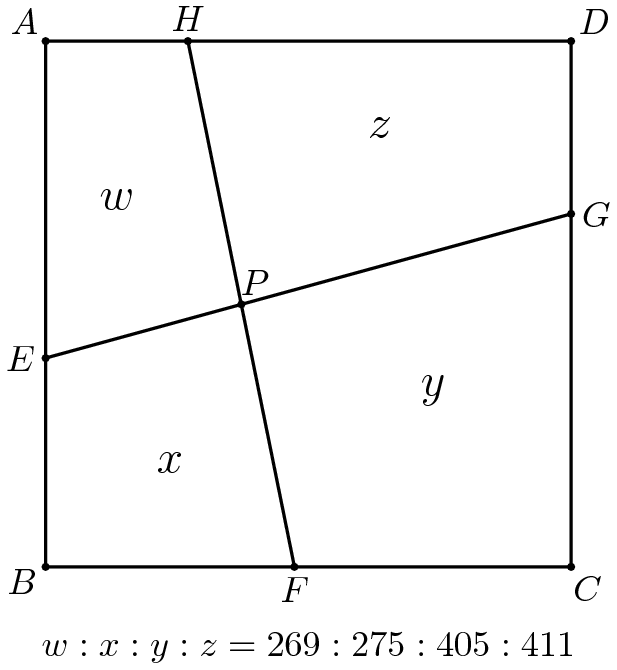
\includegraphics[width = 61.6mm]{img/fig0.png}
\end{center}